\item Na figura abaixo, estão representadas as curvas de nível (ou o diagrama de
contornos) de uma função de duas variáveis. Em relação a elas, marque a alternativa ou
alternativas que contenham as duas afirmações verdadeiras: 

\begin{center}
	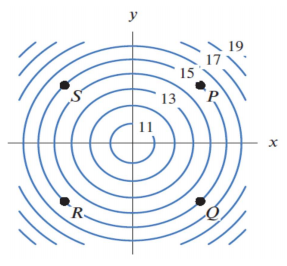
\includegraphics[scale=1]{fig1}
\end{center}

\begin{enumerate}
	\item $f_x(S) < 0$ e $f_y(R) > 0$
	\item $f_x(S) < 0$ e $f_y(R) > 0$
	\item $f_x(S) < 0$ e $f_y(R) > 0$
	\item $f_x(S) < 0$ e $f_y(R) > 0$
	\item $f_x(S) < 0$ e $f_y(R) > 0$
\end{enumerate}

\solucao

A única alternativa correta é a letra a.
